\documentclass{article}
\title{Nechyba Ch.19 扭曲性税收与补贴}
\author{Dawei Wang}
\date{\today}
\usepackage{ctex}
\usepackage{amsmath}
\usepackage{amssymb}
\usepackage{graphicx} %插入图片的宏包
\usepackage{float} %设置图片浮动位置的宏包
\usepackage{subfigure} %插入多图时用子图显示的宏包
\begin{document}
	\maketitle
税收导致无谓损失或者是无效率,这种无效率是指提高替代效应的无效率。

\section{竞争性市场中的税收与补贴}
几乎所有的税收都会改变经济中的一些机会成本。换句话说,几乎所有的税收都在一定情况下扭曲了市场价格,而使市场的各方达到一个均衡的产出。

税收和补贴的作用在改变价格方面是非常类似的。实际上,我们可以把补贴当作负的税收。

\subsection{谁支付税收以及谁收到补贴}
政府可以通过制定法律条文的方法,使得买方在买征税物品时向政府缴税。同样地,政府可以规定条文使得卖方缴税,或者是使双方都缴税。

\hspace*{\fill}

法定归宿与经济归宿

法定归宿表示法律规定中应负责缴纳税金的人是谁。

经济归宿是指当税负出现,达到均衡时,买方和卖方的实际税负负担。

\begin{figure}[H] %H为当前位置,!htb为忽略美学标准,htbp为浮动图形
	\centering %图片居中
	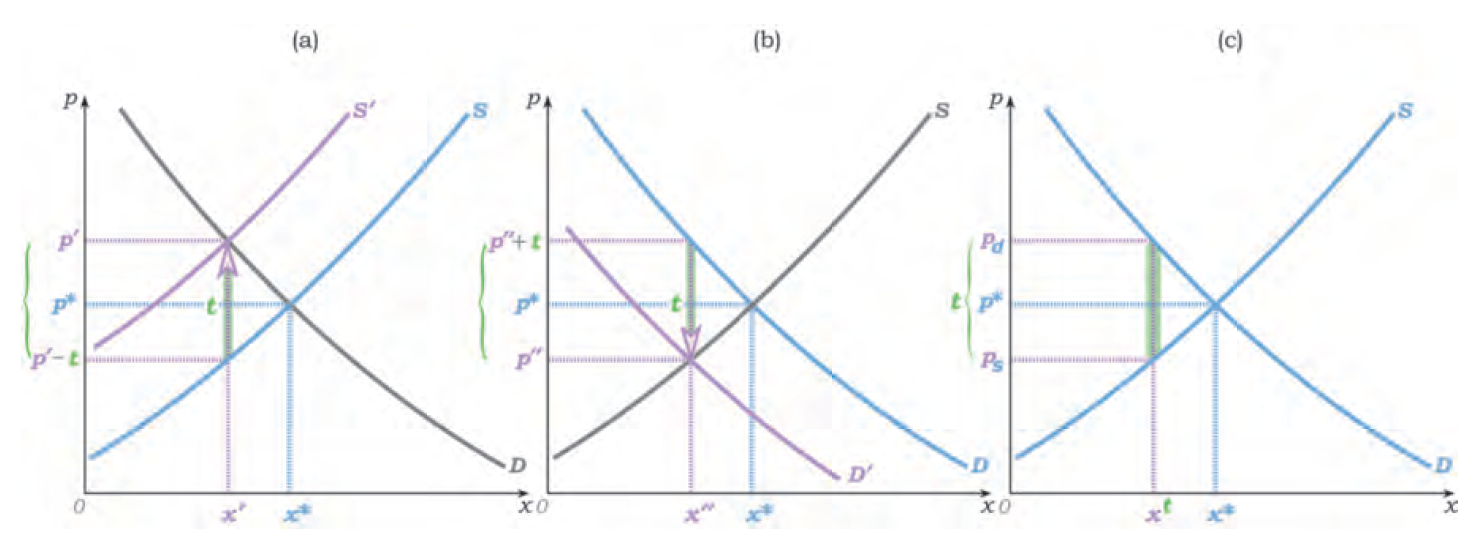
\includegraphics[width=1\textwidth]{19_1} %插入图片,[]中设置图片大小,{}中是图片文件名
	\caption{Statutory versus Economic Incidence of Taxes} %最终文档中希望显示的图片标题
	\label{Fig.main2} %用于文内引用的标签
\end{figure}

如果对每一单位产品x都向生产者征税t,从法定归宿上说,每生产一单位x,厂商就负担税负t。如此就提高了边际成本,幅度为t,市场中每个厂商的MC曲线都会上升。短期内,市场中的供给曲线是所有MC曲线的加总,这就意味着短期市场供给曲线会上升t。与此类似,由于长期市场供给曲线取决于AC曲线的最低点,因此,长期市场供给曲线也会上升t。

现在假设政府转而向消费者征收x的单位税,这种情况下,生产者成本保持不变,但是以往愿意支付p价格的消费者在知道他必须向政府支出t单位税后,现在只愿意支付(p-t)的价格。因此,需求曲线将会下降t。

因此虽然二者的法定归宿不同,但经济归宿相同,都将在买方支付价格与卖方收到价格相差t时达到均衡。无论法律条文规定税负怎样支付以及是由哪一方承担,税收的经济归宿是一样的,即买方和卖方共同承担征税的负担,买方比先前支付更高的价格,而卖方得到的收入则比以前少。由于可以将补贴看作负的税收,因此补贴的效果也可以这样分析。


\hspace*{\fill}

经济归宿与价格弹性

税收和补贴的经济归宿取决于买方和卖方对价格变动的相关反应。相对弹性小,承税(补贴)高。

\hspace*{\fill}

\begin{figure}[H] %H为当前位置,!htb为忽略美学标准,htbp为浮动图形
	\centering %图片居中
	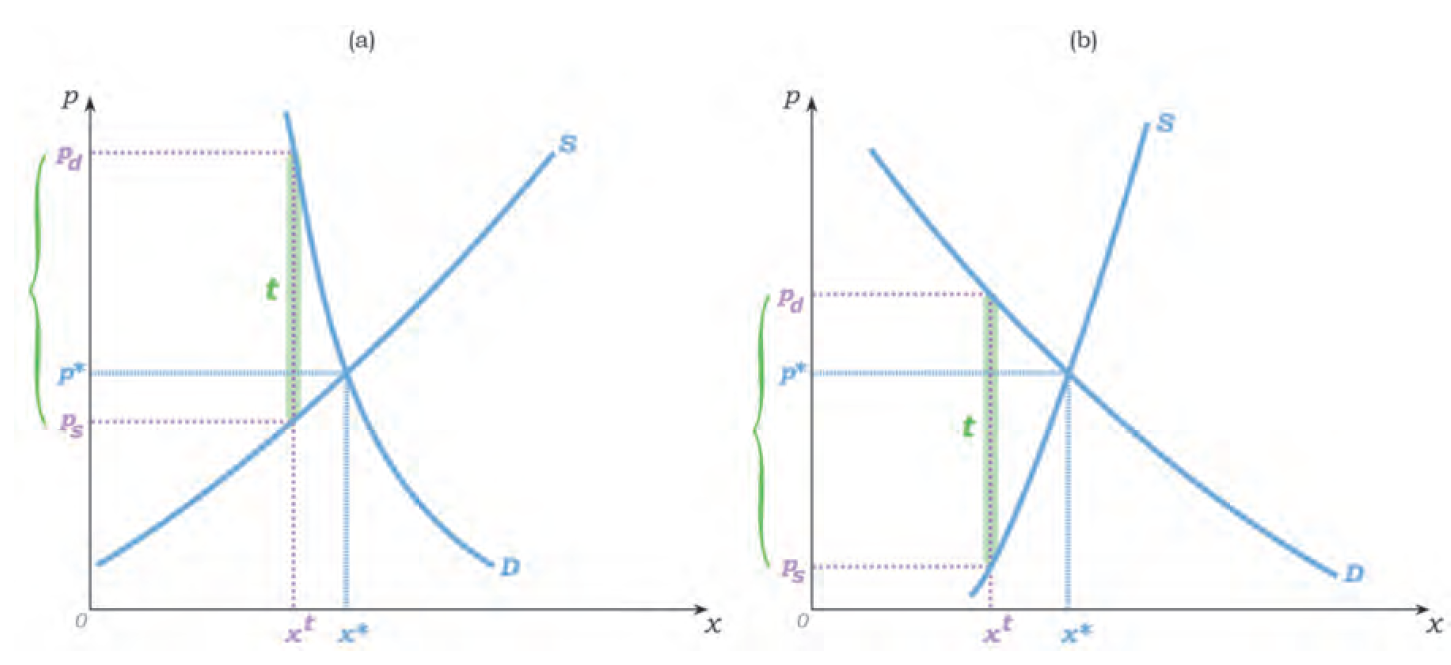
\includegraphics[width=1\textwidth]{19_2} %插入图片,[]中设置图片大小,{}中是图片文件名
	\caption{Price Elasticities and the Relative Burden of Taxes on Buyers and Sellers} %最终文档中希望显示的图片标题
	\label{Fig.main3} %用于文内引用的标签
\end{figure}

\hspace*{\fill}

征税对市场产出和税收收入的影响

价格弹性决定了哪一方会多承担税收的负担,还决定了有多少市场产出会对税收变化作出反应以及税收收入会提高多少。


\begin{figure}[H] %H为当前位置,!htb为忽略美学标准,htbp为浮动图形
	\centering %图片居中
	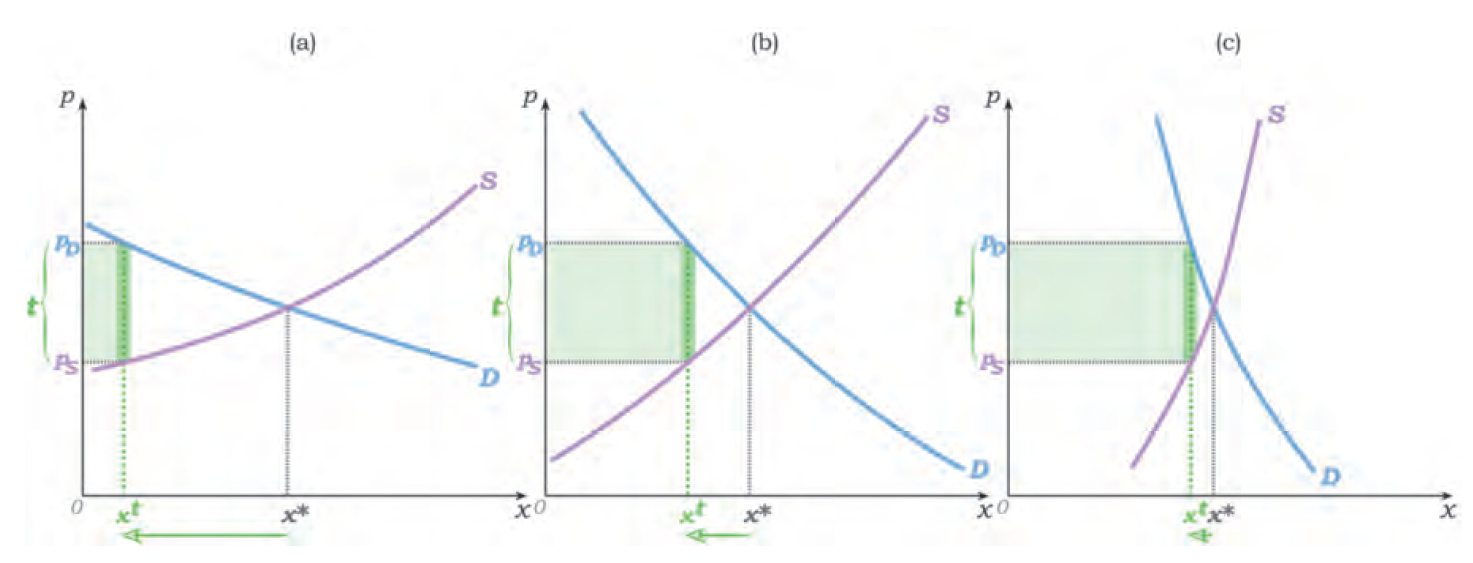
\includegraphics[width=1\textwidth]{19_3} %插入图片,[]中设置图片大小,{}中是图片文件名
	\caption{Taxes and Market Output as Economic Agents Become More Price-Responsive} %最终文档中希望显示的图片标题
	\label{Fig.main4} %用于文内引用的标签
\end{figure}

经济直觉为:如果消费者和生产者对价格变化十分敏感,他们对征税的反应会减少政府的收入。

\hspace*{\fill}

税收对其他市场的差异化影响

以上分析都是建立于局部分析的基础上——简单假设其他商品价格都是固定的且其他的商品也是没有被征税的。然而经常发生这种情况:当对一个市场征税时,通常会对其他市场造成不同程度的影响。

当考虑对那些已经存在很多税收的市场征收新的税种或是提高已有税种的税收时,对其他市场的次级影响可能比对原先市场的初始影响还大。

\subsection{重温税收的净损失}
市场需求和供给曲线是有价格变化导致的预期行为变化的充分描述。

\hspace*{\fill}

当偏好是拟线性时,由于税收和补贴而引起的无谓损失

\begin{figure}[H] %H为当前位置,!htb为忽略美学标准,htbp为浮动图形
	\centering %图片居中
	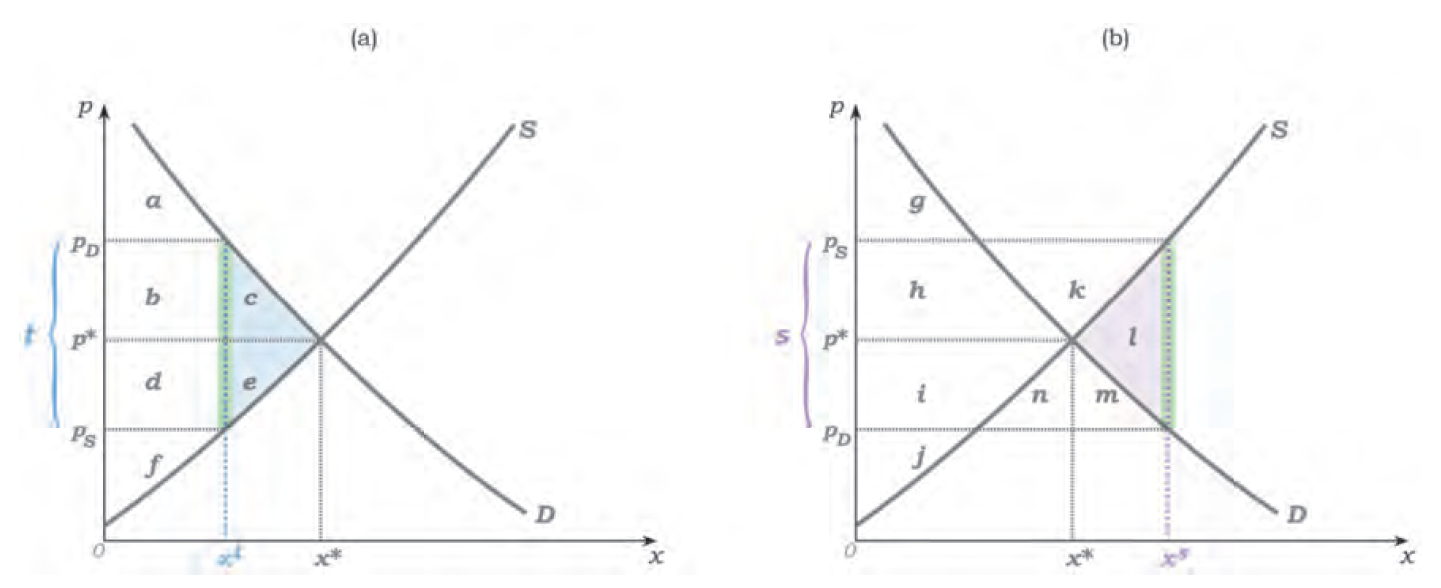
\includegraphics[width=1\textwidth]{19_4} %插入图片,[]中设置图片大小,{}中是图片文件名
	\caption{Deadweight Loss when Tastes Are Quasilinear} %最终文档中希望显示的图片标题
	\label{Fig.main5} %用于文内引用的标签
\end{figure}

税收或补贴导致的无谓损失可以看作是和市场均衡相关的三角形。当需求和供给变得更加无弹性时,三角形就变小了。实际上,如果需求和供给曲线中的一个是完全无弹性的话,无谓损失就会消失,这时税收就是有效率的。而由补贴导致的无谓损失也是一样的情况。

\hspace*{\fill}

劳动市场和资本市场的无谓损失

政府的大部分税收收入都来自收入税,这些收入来自劳动或投资(比如储蓄)。这些税收会改变线下的机会成本或现在还是将来消费的机会成本。当对劳动收入征税时就会改变闲暇的机会成本,当对储蓄收税时就改变未来消费或现在消费的机会成本。

当劳动供给无弹性,如果政府在这个时候对每小时劳动征税t,这不会对工人的工作时间产生影响,雇主付给工人的小时工资也不会变化。然而,由于劳动供给的无弹性,工人将会承担所有的税收负担,其税后工资为$ (w^*-t) $。

\begin{figure}[H] %H为当前位置,!htb为忽略美学标准,htbp为浮动图形
	\centering %图片居中
	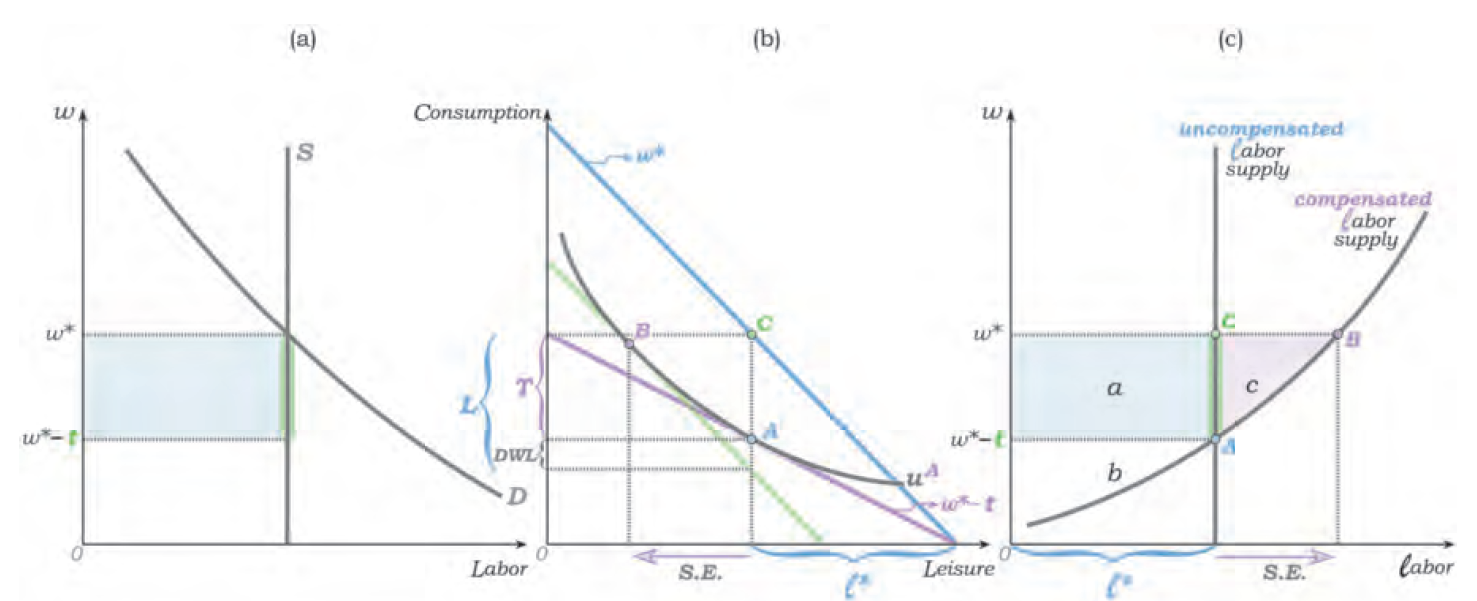
\includegraphics[width=1\textwidth]{19_5} %插入图片,[]中设置图片大小,{}中是图片文件名
	\caption{Deadweight Loss from Wage Taxes when Labor Supply Is Perfectly Inelastic} %最终文档中希望显示的图片标题
	\label{Fig.main6} %用于文内引用的标签
\end{figure}

看起来不存在无谓损失,实际上是存在的,而且一定是对工人施加的,因为 生产者支付的工资不受税收的影响。

在图(b)中,总的税收提高收入为L,而工资税收提高收入为T,这意味着存在着无谓损失,在图中表现为DWL。

在图(c)中工人剩余可用补偿劳动供给曲线来衡量,税后剩余为(b)。若在一次总量税条件下使工人获得同样的效用,则这一点是B点,此时工资为$ w^* $。工人剩余为$ (a+b+c) $,比A点的税后剩余大$ (a+c) $。然而,在A点工人已经支付了工资税(a),而在B点我们则没有把这个工人已经支付了总量税从而使得他们与在A点有相同效用的事实考虑进去。工资税与一次总量税收入的差即为无谓损失(c)。

劳动供给并不总是完全无弹性的,它有时候甚至是向下倾斜的,但是替代效应总是意味着补偿劳动供给曲线总是向上倾斜的。因此,无论我们在劳动市场均衡中是否看得到,只有闲暇和消费存在替代性,工资税就总是会有无谓损失,而闲暇和消费的替代性几乎必然存在。

\hspace*{\fill}

补贴造成的劳动或资本市场的无谓损失

\begin{figure}[H] %H为当前位置,!htb为忽略美学标准,htbp为浮动图形
	\centering %图片居中
	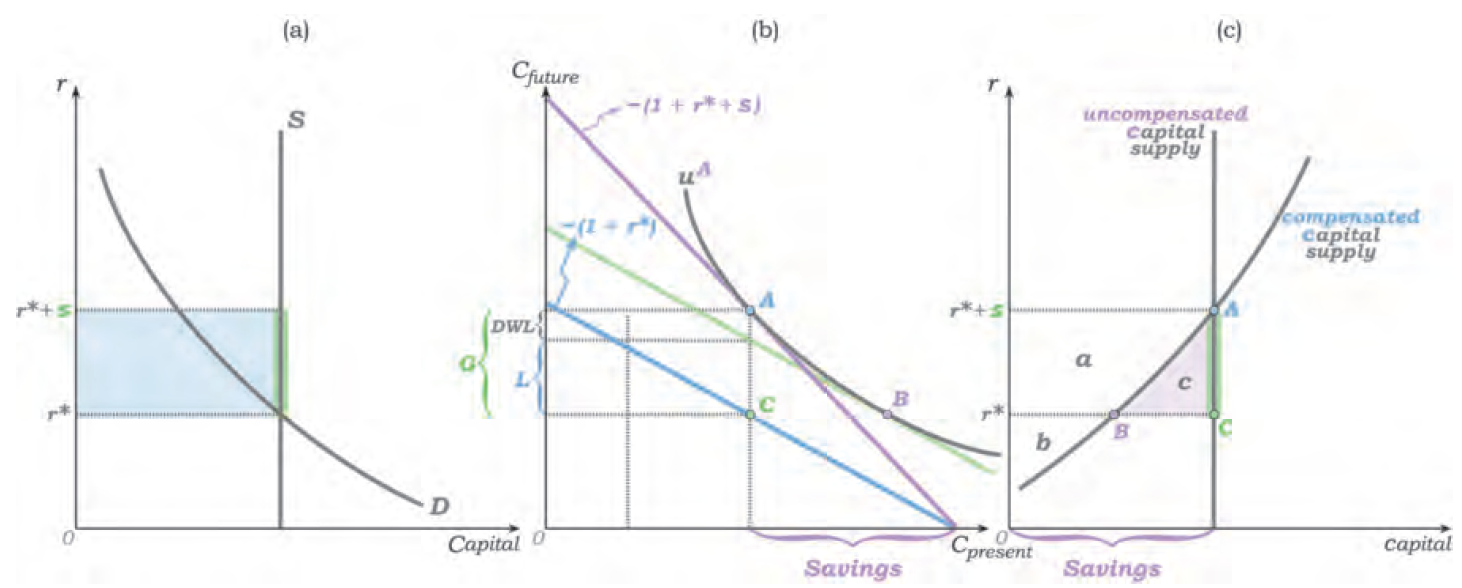
\includegraphics[width=1\textwidth]{19_6} %插入图片,[]中设置图片大小,{}中是图片文件名
	\caption{Deadweight Loss from Subsidies for Saving when Saving Behavior Is Perfectly Inelastic} %最终文档中希望显示的图片标题
	\label{Fig.main7} %用于文内引用的标签
\end{figure}

工资税:得到的工资比支付的少;工资补贴:得到的工资比支付的多。

政府由于补贴而对单个储蓄者支付的成本可以用A和C之间的垂直距离衡量,即为G。通过观察上面的实预算线和下面的虚预算线的差别,我们可以知道仅仅补贴L就可以使这个人和在政府支付数量为G的扭曲性补贴时的状况一样好。G和L之差即为对单个储蓄者的无谓损失。

通过补偿资本供给曲线,我们可以知道在扭曲性补贴下储蓄者剩余为$ (a+b) $,在一次总量补贴下仅为(b)。由于储蓄者在A点和B点的满足感是相同的,B点的加总补贴一定等于(a)。但是扭曲性补贴花费(a+c),其中比加总补贴大(c)。

\hspace*{\fill}

当税率提高时的无谓损失和税收收入

\begin{figure}[H] %H为当前位置,!htb为忽略美学标准,htbp为浮动图形
	\centering %图片居中
	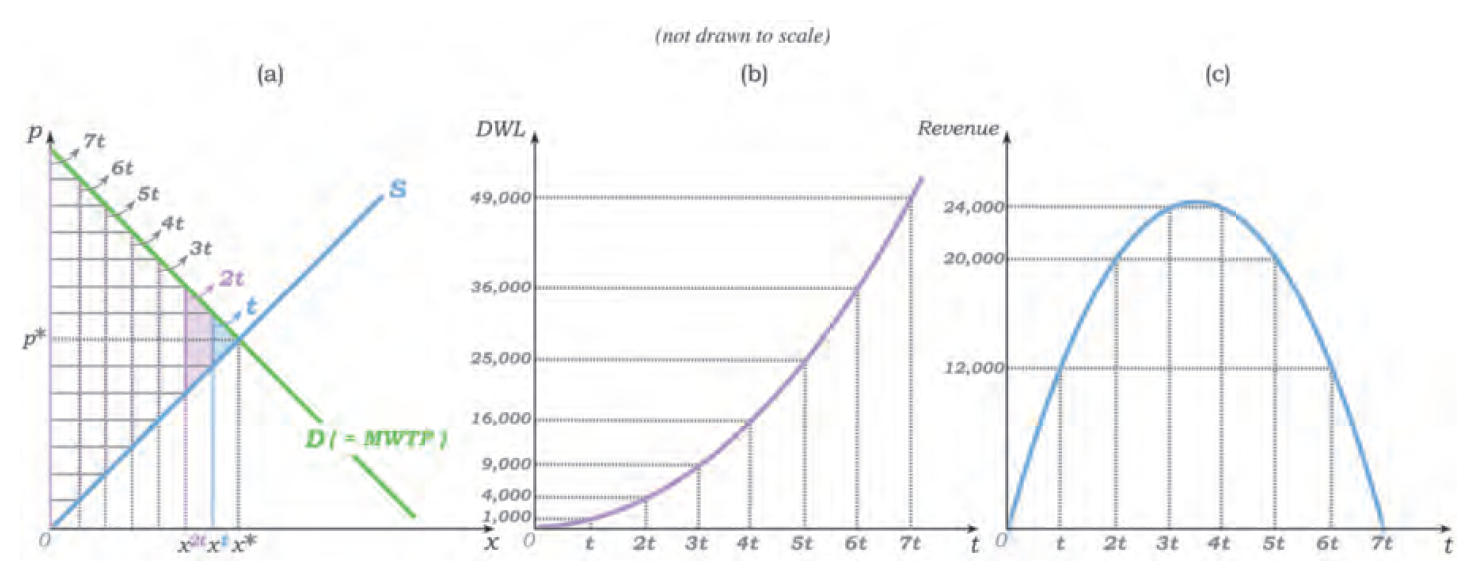
\includegraphics[width=1\textwidth]{19_7} %插入图片,[]中设置图片大小,{}中是图片文件名
	\caption{Deadweight Loss and Tax Revenue when Tastes Are Quasilinear} %最终文档中希望显示的图片标题
	\label{Fig.main8} %用于文内引用的标签
\end{figure}

当拥有线性需求和供给曲线时,当税率增加k,则无谓损失增加$ k^2 $。

税率和税收收入的关系:当没有征税时,税收收入为0,当税率足够大时,税收收入再次为0.

在大税基的情况下征收低税率比在小税基下征收高税率更有效率。

\subsection{对土地征税:有效的现实世界税收}

需求或供给曲线不可能足够地无弹性以使得税收是有效率的,因为无价格弹性的行为关系会很好地掩饰潜在的替代效应。

土地价值即土地的市场价格,而地租则来自一定数量的土地在一段时间的收入。土地拥有价值的原因是土地拥有者可以每年从土地上获取地租。土地的特殊之处在于,它不是生产出来的,因此它的供给是固定的。

使用土地的机会成本是将土地租给别人所获得的收入。租金取决于土地的质量和别人的支付能力。

土地价值LV和土地租金的关系为:

\[
LV=\frac{LR}{1+r}+\frac{LR}{(1+r)^2}+\cdots=\frac{LR}{r}
\]

\hspace*{\fill}

土地租金的税收

假设政府给土地租金施加t的税,由于土地的价值等于所有未来土地租金的和的现值。因此土地价值瞬间从LV下降到(1-t)LV。

这种税收无法避免,不可能出现替代效应以使得征税无效率。土地租金税收是将财富从土地所有者到政府的一个简单转移。土地拥有者的财富减少了,而政府拥有了所有土地拥有者丧失的财富。

\subsection{一般均衡VS局部均衡税收归宿}

税收规定在哪一方征税影响不大,因为哪方最终承担了税收取决于需求和供给曲线的相对弹性。税负可能从卖方转移给买方,也可能从买方转移给卖方,这都取决于谁的经济行为更加缺乏弹性。

然而,税负的转移不仅仅局限在被征税的这个市场的活动者当中。在很多情况下,税负会转移出被征税的市场而到达那些没有法律税负义务的市场的活动者身上。当这种情况发生时,就不仅存在我们已经分析过的局部均衡影响,还存在一般均衡税收归宿影响。

税收的一般均衡影响非常重要,这也因此大大增加了税收政策的复杂性。

\section{期望效用与独立性公理}

独立性公理是构建期望效用理论的基石。

独立性公理假设如下:假定存在三个赌局,$ G_1,G_2,G_3 $。那么

\[
G_1\succeq G_2, if\enspace  and\enspace only\enspace if \enspace (\alpha G_1+(1-\alpha)G_3)\succeq(\alpha G_2+(1-\alpha)G_3)
\]

用文字表达即:赌局1偏好于赌局2当且仅当赌局1与赌局3的混合比赌局2与赌局3的相同混合受偏好。从而,当这些赌局与任何一个其他赌局混在一起时,一个个体对两个赌局的偏好保持相同,或者,换言之,一个个体对两种赌局的偏好独立于所混合的其他赌局(只要它们以相同的方式混合在一起)。

\hspace*{\fill}

如果一个个体对赌局的偏好满足独立性公理,这些偏好就能由期望效用函数表示。

\section{Allais Paradox与后悔理论}

在面对极小概率事件时,独立性公理可能并不成立(人们会后悔)。


	
	
\end{document}